% Self-contained Beamer source. Compile with pdfLaTeX, twice.
% No external figures, bibliography file, or thesis file are needed to compile.
% PRIVATE OPPONENT NOTES are stored in \note{...} throughout this file.
% To print them, replace hide notes below with show notes, or
% show notes on second screen=right. The delivered PDF hides these notes.
% Source: Thesis_David_Cardona.pdf supplied by the principal opponent.
% Thesis Arabic printed page n corresponds to PDF page n+14.
% Assessment concerns the manuscript and reported calculations; no code was rerun.
\documentclass[aspectratio=169,11pt]{beamer}
\usepackage[T1]{fontenc}
\usepackage[utf8]{inputenc}
\usepackage{lmodern}
\usepackage{amsmath,amssymb,booktabs,array}
\usepackage{pgfplots}
\pgfplotsset{compat=1.18}
\usefonttheme{professionalfonts}
\setbeameroption{hide notes}

\definecolor{navy}{HTML}{17324D}
\definecolor{teal}{HTML}{007F86}
\definecolor{ink}{HTML}{253746}
\definecolor{muted}{HTML}{60717C}
\definecolor{paper}{HTML}{F2F6F8}
\definecolor{rust}{HTML}{9D4930}
\setbeamercolor{normal text}{fg=ink,bg=white}
\setbeamercolor{structure}{fg=teal}
\setbeamercolor{frametitle}{fg=navy,bg=white}
\setbeamerfont{frametitle}{size=\Large,series=\bfseries}
\setbeamercolor{title}{fg=navy}
\setbeamerfont{title}{size=\LARGE,series=\bfseries}
\setbeamercolor{block title}{fg=navy,bg=paper}
\setbeamercolor{block body}{fg=ink,bg=paper}
\setbeamercolor{alerted text}{fg=rust}
\setbeamertemplate{navigation symbols}{}
\setbeamertemplate{itemize items}[circle]
\setbeamersize{text margin left=8mm,text margin right=8mm}
\setbeamertemplate{frametitle}{\vspace{3mm}\insertframetitle\par\vspace{1mm}{\color{teal}\hrule height 0.5pt}\vspace{2mm}}
\setbeamertemplate{footline}{%
  \leavevmode\hbox{%
  \begin{beamercolorbox}[wd=.84\paperwidth,ht=2.8ex,dp=1.3ex,leftskip=8mm]{normal text}
    \color{muted}\scriptsize Cardona Ochoa\quad|\quad Principal opponent briefing
  \end{beamercolorbox}%
  \begin{beamercolorbox}[wd=.16\paperwidth,ht=2.8ex,dp=1.3ex,rightskip=8mm]{normal text}
    \hfill\color{muted}\scriptsize\insertframenumber/\inserttotalframenumber
  \end{beamercolorbox}}}
\newcommand{\nuc}[2]{\ensuremath{{}^{#1}\mathrm{#2}}}
\newcommand{\EP}{\mathrm{EP}}
\newcommand{\src}[1]{\par\vfill{\color{muted}\fontsize{7.5}{9}\selectfont\textit{Source:} #1\par}}
\newcommand{\takeaway}[1]{\par\medskip{\color{navy}\bfseries #1}\par}
\newcommand{\qtitle}[2]{\par\textbf{\color{teal}#1. #2}\par\smallskip}
\newcommand{\spacer}{\vspace{2mm}}
\hypersetup{colorlinks=true,urlcolor=teal,linkcolor=navy,
  pdftitle={David Cardona Ochoa: Scientific assessment and defence questions},
  pdfauthor={Principal opponent briefing},pdfsubject={Continuum coupling, exceptional points and light nuclei}}

\title{Scientific assessment and defence questions}
\subtitle{David Cardona Ochoa\\[2mm]
\normalsize Systematics studies of the continuum-coupling correlations\\
in near-threshold states}
\author{Briefing for the principal opponent}
\institute{Universit\'e de Caen Normandie\quad\textbullet\quad GANIL}
\date{Manuscript dated 11 August 2026\\[1mm]\small Review prepared 7 October 2026}

\begin{document}

\begin{frame}
\titlepage
\note{This is an independent reading of the final PDF supplied by the opponent. The title and institution follow the thesis cover. The briefing is intended to support, rather than replace, the opponent's judgement. It does not certify the numerical implementation, unpublished code, or candidate's individual contribution.}
\end{frame}

\begin{frame}{Principal assessment}
\begin{itemize}\setlength\itemsep{3mm}
\item A substantial microscopic study of how the continuum reorganises nuclear resonances, decay channels and time evolution.
\item The strongest result is the consistent identification of exceptional points in parameter-tuned GSM--CC Hamiltonians.
\item The \nuc{4}{He} calculations add a valuable study of negative-parity resonances and threshold sensitivity.
\item The main reservations concern quantitative validation, fitted corrections, physical interpretation of survival curves, and the definition of correlation energy.
\end{itemize}
\takeaway{The work supports a strong doctoral discussion; several physical claims need narrower wording or further evidence.}
\src{Thesis, Introduction; Ch. 3, pp. 100--155; Conclusions, pp. 156--159.}
\note{Lead with the achievements. The diagnostics establish exceptional points of the calculated Hamiltonians convincingly. The weak point is the passage from those tuned models to a unique experimental interpretation. The helium work is valuable even where branchings fail: those failures identify physics missing from the present channel space. This is a scientific assessment, not a formal recommendation on acceptance; that also requires the defence, institutional criteria and assessment of the candidate's own contribution.}
\end{frame}

\begin{frame}{What the thesis actually establishes}
\small
\renewcommand{\arraystretch}{1.15}
\begin{tabular}{>{\raggedright\arraybackslash}p{.19\textwidth}>{\raggedright\arraybackslash}p{.43\textwidth}>{\raggedright\arraybackslash}p{.29\textwidth}}
\toprule
System & Main finding & Evidential status\\\midrule
\nuc{6}{Li}, $2^+$ & EP topology; finite paired strength; split peak & Strong in the tuned model\\
\nuc{7}{Li}/\nuc{7}{Be}, $5/2^-$ & Mirror-channel comparison; width bifurcation & Strong diagnostics; physical relevance open\\
\nuc{8}{Be}, $2^+$ & EP and proton/$\alpha$ width redistribution & Threshold and EP effects intertwined\\
Prepared resonances & Polynomial envelope; late-time tails & Preparation and asymptotics need checks\\
\nuc{4}{He} & Threshold alignment; nonrigid energy response & Clear sensitivity; interpretation open\\\bottomrule
\end{tabular}
\src{Thesis, \S\S3.1--3.4. ``Strong'' here describes support in the reported calculations, not an observed EP in a physical nucleus.}
\note{The contribution is the microscopic coupled-channel realisation and comparison across nuclei. EPs, resonance trapping and non-exponential decay were known before this thesis. The thesis cites earlier work on the beryllium doublet. Ask the candidate to distinguish personal conceptual contributions, implementation work, and inherited framework.}
\end{frame}

\begin{frame}{Method: a common structure and reaction framework}
\begin{columns}[T]
\begin{column}{.49\textwidth}
\textbf{Gamow shell model, coupled channels}
\begin{itemize}\setlength\itemsep{2mm}
\item Berggren basis: bound states, resonance poles and nonresonant continuum.
\item Antisymmetrised cluster channels and outgoing boundary conditions.
\item Complex poles $z=E_r-i\Gamma/2$ connect spectra and decay.
\end{itemize}
\end{column}
\begin{column}{.47\textwidth}
\textbf{Two implementations}
\begin{itemize}\setlength\itemsep{2mm}
\item Inert \nuc{4}{He} core for lithium and beryllium; effective interactions and channel corrections.
\item No-core GSM--CC for \nuc{4}{He}, with HO internal states and continuum relative motion.
\item Thresholds, channel truncations and calibration choices matter in both.
\end{itemize}
\end{column}
\end{columns}
\takeaway{Major strength: structure, scattering and decay are treated in a shared many-body framework.}
\src{Thesis, Ch. 2, pp. 18--69; model definitions, pp. 103, 116--117, 134, 138--140.}
\note{GSM--CC provides a particularly direct microscopic description of continuum coupling. Avoid describing it as the only formalism capable of resonance interference or double poles. A general multilevel scattering description is broader than a sum of isolated Breit--Wigner peaks. The inert-core and no-core calculations have different calibration and truncation issues.}
\end{frame}

\begin{frame}{Exceptional points: complementary diagnostics}
\begin{columns}[T]
\begin{column}{.51\textwidth}
\begin{itemize}\setlength\itemsep{2mm}
\item Two complex eigenvalues and their eigenvectors coalesce.
\item Local splitting has square-root structure:
\[z_\pm-z_{\EP}\sim\pm\sqrt{a\,\delta V_p+b\,\delta V_n}.\]
\item Phase rigidity tends to zero.
\item A loop around the \nuc{6}{Li} EP exchanges eigenvalue sheets.
\end{itemize}
\end{column}
\begin{column}{.45\textwidth}
\textbf{Why this is persuasive}
\spacer
\par Agreement among eigenvalue, eigenvector and topological tests is much stronger than a near-degeneracy alone.
\medskip
\textbf{What remains to quantify}
\spacer
\par Numerical tolerance, contour and channel-space stability, and sensitivity to alternative acceptable interactions.
\end{column}
\end{columns}
\src{Thesis, pp. 79--94; Figs. 3.3--3.5, 3.13--3.17, 3.33--3.34.}
\note{Defectiveness is essential: a degeneracy with two independent eigenvectors is not an EP. For a generic second-order EP, two real controls are appropriate. Ask how phase rigidity is evaluated near self-orthogonality, what resolution distinguishes numerical zero from a small value, and whether the double-pole residue or a Jordan chain was directly constructed.}
\end{frame}

\begin{frame}{The EPs found by varying two spin--orbit strengths}
\small
\renewcommand{\arraystretch}{1.45}
\begin{center}
\begin{tabular}{lrrrr}
\toprule
System & $J^\pi$ & $V_{\rm SO}^{\ell=1}(p)$ & $V_{\rm SO}^{\ell=1}(n)$ & $\Gamma_{\EP}$\\
 & & MeV & MeV & keV\\\midrule
\nuc{6}{Li} & $2^+$ & 8.463 & 7.801 & 111\\
\nuc{7}{Li} & $5/2^-$ & 5.67 & 4.97 & $\simeq477$\\
\nuc{7}{Be} & $5/2^-$ & 4.38 & 4.48 & 477\\
\nuc{8}{Be} & $2^+$ & 2.2640 & 1.9116 & $\simeq99$\\\bottomrule
\end{tabular}
\end{center}
\medskip
These are locations in \textbf{Hamiltonian parameter space}. They are not laboratory control settings or measured degeneracies.
\takeaway{The nearly equal mirror widths are a numerical result after separate retuning, rather than a protected mirror-symmetry identity.}
\src{Thesis, pp. 105--106, 117--120, 136. \nuc{7}{Li} is also quoted as 476 keV elsewhere.}
\note{Energy origins differ from reaction centre-of-mass energies, so this overview deliberately compares control parameters and widths rather than absolute energies across systems. The source quotes the beryllium width approximately; do not infer more precision than reported. Physical relevance depends on distance from the calibrated Hamiltonian and uncertainty in that calibration.}
\end{frame}

\begin{frame}{\nuc{6}{Li}: a clear microscopic EP demonstration}
\begin{itemize}\setlength\itemsep{3mm}
\item The starting $2^+$ poles have $(E,\Gamma)=(0.234\,\mathrm{MeV},168\,\mathrm{keV})$ and $(1.282\,\mathrm{MeV},95\,\mathrm{keV})$.
\item At the EP: $E=0.564$ MeV and $\Gamma=111$ keV; energies are relative to the \nuc{4}{He} core.
\item Loop exchange, square-root trajectories and vanishing rigidity support the identification.
\item Individual spectroscopic factors diverge with opposing contributions; their paired sum stays finite.
\item Calculated elastic scattering has a split peak; intermediate-time EP survival has a polynomial prefactor.
\end{itemize}
\src{Thesis, pp. 105--114; Figs. 3.3--3.7 and 3.10.}
\note{The divergent quantities are biorthogonally normalised pole-state diagnostics. The finite paired sum is consistent with treating the coalescing subspace together; it is not by itself a measured transition strength. The scattering and time curves are for the retuned Hamiltonian. Their physical interpretation is a further step beyond the mathematical diagnosis.}
\end{frame}

\begin{frame}{\nuc{6}{Li}: physical calibration is the weak point}
\begin{columns}[T]
\begin{column}{.46\textwidth}
\textbf{Widths at the starting Hamiltonian}
\medskip
\small\renewcommand{\arraystretch}{1.4}
\begin{tabular}{lrr}
\toprule
 & Experiment & GSM--CC\\
 & keV & keV\\\midrule
$2^+_1$ & 1300 & 168\\
$2^+_2$ & 541 & 95\\\bottomrule
\end{tabular}
\medskip
\par Underestimated by factors $7.7$ and $5.7$.
\par Width ratio: $2.40$ versus $1.77$.
\end{column}
\begin{column}{.50\textwidth}
\textbf{Distance to the EP}
\spacer
\par The starting spin--orbit strengths are $3.492$ MeV for protons and $3.936$ MeV for neutrons.
\medskip
\par The EP requires increases by factors $2.42$ and $1.98$.
\medskip
\par\textbf{Assessment}
\spacer
\par Robust EP evidence in the continued model; quantitatively realistic signatures for physical \nuc{6}{Li} are less established.
\end{column}
\end{columns}
\src{Thesis, Table 3.1, p. 103; Fig. 3.2, p. 104; discussion, p. 106. Experimental values as quoted by the thesis.}
\note{The text's claim that the width ratio is correctly reproduced is too strong: the ratio differs by about 26 percent. This does not invalidate the EP of the model. It does limit extrapolation to physical pole positions and cross sections. Ask which conclusions survive alternative fits that improve the widths, and whether the EP remains comparably close in a statistically meaningful parameter metric.}
\end{frame}

\begin{frame}{\nuc{7}{Li} and \nuc{7}{Be}: the mirror comparison}
\small\renewcommand{\arraystretch}{1.4}
\begin{tabular}{p{.21\textwidth}p{.35\textwidth}p{.35\textwidth}}
\toprule
 & \nuc{7}{Li} & \nuc{7}{Be}\\\midrule
Doublet & $5/2^-_1,5/2^-_2$ & $5/2^-_1,5/2^-_2$\\
Open channels at EP & $\alpha+t$ & $\alpha+\nuc{3}{He}$ and $p+\nuc{6}{Li}$\\
Pole at EP & $E=-4.023$ MeV, $\Gamma\simeq477$ keV & $E=-2.36$ MeV, $\Gamma=477$ keV\\
Scattering response & Clear split peak in the single open channel & Dominant cluster channel retains a weaker split peak; proton response suppressed\\\bottomrule
\end{tabular}
\medskip
\par At the \nuc{7}{Be} EP, the \nuc{3}{He} partial width is approximately ten times the proton partial width.
\takeaway{Open-channel composition controls how the same pole singularity appears in different reactions.}
\src{Thesis, pp. 117--127; Figs. 3.13--3.17 and 3.22--3.23. Energies use the model's Hamiltonian origin.}
\note{A useful comparison because the topology of a second-order EP persists but its projection into particular channels changes. The fits are not identical mirror Hamiltonians: Coulomb, thresholds and channel correction factors differ. Avoid interpreting the equal EP widths as exact symmetry. The plotted charged-particle cross sections include Rutherford normalization; the scattering angle and background treatment should be specified for an experimental proposal.}
\end{frame}

\begin{frame}{Mirror nuclei: singular pole strengths, regular subspace}
\begin{itemize}\setlength\itemsep{3mm}
\item Individual complex spectroscopic factors show singular real and imaginary parts as the two states coalesce.
\item Their summed contributions remain finite, removing the singularity associated with separating the two pole states.
\item Electromagnetic $B(E2)$ quantities exhibit related singular behaviour near the EP.
\item This is valuable evidence of the breakdown of an isolated-state description.
\end{itemize}
\takeaway{A physical response must combine the coalescing subspace, interference and continuum; a divergent pole strength is not an infinite measured transition rate.}
\src{Thesis, pp. 121--125; Figs. 3.18--3.21.}
\note{The thesis generally handles the normalization issue thoughtfully. Ask the candidate to build an explicitly finite response to an electromagnetic probe, with the correct metric and complete continuum. Spectroscopic factors themselves are representation-dependent, while cross sections and suitably defined response functions are the experimental targets.}
\end{frame}

\begin{frame}{Width bifurcation and channel alignment}
\begin{itemize}\setlength\itemsep{3mm}
\item Trajectories connecting two EPs develop a broad and a trapped resonance.
\item In \nuc{7}{Li}, the narrow width approaches zero between the EPs.
\item In \nuc{7}{Be}, the narrow state becomes proton-decaying while the broad state aligns with the \nuc{3}{He} channel.
\item The narrow \nuc{7}{Be} state still has a finite proton width: it decouples from one channel, not the entire continuum.
\item Total-width conservation is not exact along these scans, since the spin--orbit variation also moves energies relative to thresholds.
\end{itemize}
\src{Thesis, pp. 127--130; Figs. 3.24--3.28. The second EPs are in nonphysical parameter regions.}
\note{This is one of the most illuminating results: it connects non-Hermitian eigenstate structure to partial decay widths. However, varying the potential simultaneously changes kinematics. A control with fixed thresholds/energies or a self-energy decomposition would help distinguish alignment from ordinary penetrability changes. Robustness to omitted channels is particularly relevant when a state is described as channel-pure.}
\end{frame}

\begin{frame}{Mirror nuclei: validation and experimental interpretation}
\begin{columns}[T]
\begin{column}{.44\textwidth}
\small\renewcommand{\arraystretch}{1.35}
\begin{tabular}{lrr}
\toprule
Width / keV & Experiment & Model\\\midrule
\nuc{7}{Li} $5/2^-_1$ & 880 & 729\\
\nuc{7}{Li} $5/2^-_2$ & 89 & 51\\
\nuc{7}{Be} $5/2^-_1$ & 1200 & 691\\
\nuc{7}{Be} $5/2^-_2$ & 400 & 179\\\bottomrule
\end{tabular}
\medskip
\par Especially for \nuc{7}{Be}, these are appreciable discrepancies.
\end{column}
\begin{column}{.52\textwidth}
\begin{itemize}\setlength\itemsep{2mm}
\item Cluster corrections differ between mirrors; no uncertainty band for EP coordinates is provided.
\item A split peak or a total $2\pi$ phase evolution can also arise from ordinary interfering resonances.
\item A convincing experimental claim needs pole extraction, backgrounds, channel information and uncertainties.
\end{itemize}
\end{column}
\end{columns}
\src{Thesis, Figs. 3.12 and 3.15, pp. 117, 120; model corrections, pp. 117, 119; scattering discussion, pp. 125--127.}
\note{Do not call the calculated phase change a unique EP fingerprint. The sum of phase changes from two separated poles can have the same total winding. The relevant distinction is coincident pole structure and residue behaviour in an analytically continued, constrained scattering matrix. A comparison against a non-EP two-resonance model with equivalent fit quality would make the experimental argument much stronger.}
\end{frame}

\begin{frame}{\nuc{8}{Be}: an EP and competing decay partitions}
\begin{itemize}\setlength\itemsep{3mm}
\item The well-known $2^+$ doublet near 16.6 and 16.9 MeV excitation is described with $\alpha$, proton, neutron and deuteron partitions.
\item At $V_{\rm SO}(p)=2.2640$ MeV and $V_{\rm SO}(n)=1.9116$ MeV, the poles coalesce with $\Gamma\simeq99$ keV.
\item Phase rigidity remains close to unity over much of the scan, then collapses sharply near the EP.
\item Opening $p+\nuc{7}{Li}$ redistributes width between proton and $\alpha$ decay while the total width changes little.
\end{itemize}
\takeaway{The new value is the microscopic multichannel account of the doublet, rather than the first general EP interpretation of it.}
\src{Thesis, pp. 134--138; Figs. 3.32--3.35; earlier EP treatment acknowledged on pp. 135--136.}
\note{The threshold opening and the EP occur in the same parameter study. Their causal effects should be separated by controls, not assigned to the EP solely by proximity. The plotted energy is approximately -10.612 MeV in the model origin, read from a figure; it is omitted from the main slide to avoid implying an exact tabulated value.}
\end{frame}

\begin{frame}{\nuc{8}{Be}: strengths and unresolved model dependence}
\begin{columns}[T]
\begin{column}{.47\textwidth}
\textbf{Strengths}
\begin{itemize}\setlength\itemsep{2mm}
\item Better starting width scale than in \nuc{6}{Li}: 98/97 keV versus experimental 108/74 keV.
\item Partial-width tracking gives direct reaction-channel interpretation.
\item The sharp rigidity collapse provides a useful contrast to the mirror cases.
\end{itemize}
\end{column}
\begin{column}{.49\textwidth}
\textbf{Weaknesses / checks}
\begin{itemize}\setlength\itemsep{2mm}
\item Complex channel corrections are phenomenological:
\[c(2^+)=1.0160+i0.0016.\]
\item Their effect on flux conservation and pole locations needs explanation.
\item Threshold-driven redistribution needs a non-EP comparison.
\item Channel notation and identical-$\alpha$ exchange symmetry deserve clarification.
\end{itemize}
\end{column}
\end{columns}
\src{Thesis, p. 134; Fig. 3.32, p. 135; Figs. 3.34--3.35, p. 137.}
\note{The deuteron and alpha correction is 1.0998-i0.00475. No flux violation is asserted: ask how these complex factors enter the Hamiltonian and scattering calculation and what numerical conservation checks were done. The model overestimates the second starting width (97 versus 74 keV); the blanket statement that both are underestimated is inaccurate. The channel list contains 4H instead of 4He, 3G4 instead of 1G4, and 3P3 where 3P2 is presumably intended. Odd alpha-alpha relative waves in a generic list must be excluded or explained for identical spin-zero bosons.}
\end{frame}

\begin{frame}{EP time evolution: a meaningful but conditional result}
\small
For a second-order Jordan block, $H=z_{\EP}I+N$ with $N^2=0$:
\[
 e^{-iHt/\hbar}=e^{-iz_{\EP}t/\hbar}\left(I-\frac{iNt}{\hbar}\right).
\]
For a specified preparation and projection, the pole contribution is
\[
 A_{\rm pole}(t)=(a+bt)e^{-iz_{\EP}t/\hbar},\qquad
 S_{\rm pole}(t)=|a+bt|^2e^{-\Gamma_{\EP}t/\hbar}.
\]
\begin{itemize}\setlength\itemsep{2mm}
\item The thesis finds a clear intermediate-time polynomial envelope in \nuc{6}{Li} and \nuc{7}{Li}; the \nuc{7}{Be} effect is much weaker.
\item The coefficient $b$ depends on the prepared state and its projection onto the nilpotent part.
\item The number of open channels alone does not fix the visibility of the quadratic term.
\end{itemize}
\src{Thesis, pp. 91--94, 109--115, 130--133; Figs. 3.10, 3.29--3.31. Formula includes explicit $\hbar$.}
\note{This is the pole part, not the complete survival amplitude: background and branch-cut contributions cause short- and long-time deviations. The initial packet is a Fermi-cutoff Gamow state, not necessarily a state produced in a specific reaction. A weak b can arise from projection and preparation even at a genuine EP. The 470-keV guides in mirror figures may be fitted effective slopes, rather than typographical errors; ask for the fitted coefficients, interval and units. Near an EP, diagonalising a nonnormal matrix is ill-conditioned, and at the EP it is defective. A stable exponential or Jordan-chain calculation and a real-energy cross-check are important.}
\end{frame}

\begin{frame}{Survival calculations: preparation and positivity}
\begin{columns}[T]
\begin{column}{.50\textwidth}
\textbf{What is shown}
\begin{itemize}\setlength\itemsep{2mm}
\item Cutoff radii 10, 20 and 60 fm give different reconstructed spectra and late-time strengths.
\item Broad short-, intermediate- and late-time regimes persist.
\item Some reconstructed spectral functions become negative.
\end{itemize}
\end{column}
\begin{column}{.46\textwidth}
\textbf{What must be established}
\begin{itemize}\setlength\itemsep{2mm}
\item For physical unitary evolution,
\[\rho_\Psi(E)=\sum_c|\langle E,c|\Psi\rangle|^2\geq0.\]
\item Is the plotted function this density or a projected non-Hermitian response?
\item Normalising $A(0)$ alone does not establish physical evolution for all $t$.
\end{itemize}
\end{column}
\end{columns}
\takeaway{A quantitative preparation plateau and a real-energy cross-check would strengthen the time-domain conclusions.}
\src{Thesis, Eqs. 2.142, 2.158--2.160; pp. 109--112, Figs. 3.8--3.9. Wang et al. (2023), \href{https://arxiv.org/html/2211.11619}{Sec. II}.}
\note{The positive spectral representation assumes a normalised state and Hermitian full Hamiltonian. A finite projected non-Hermitian calculation may not reproduce it automatically. Negative reconstructed density may reflect incomplete continuum representation, Fourier-window errors or a quantity with a different physical meaning. Do not conclude that all time curves are invalid. The manuscript needs to identify the cause and verify the reported regime. A nearby cutoff/diffuseness scan is more informative than only widely separated radii, whose tail strengths differ by orders of magnitude. A coherent two-pole autocorrelation also contains interference terms unless averaging or a negligible-interference approximation is invoked.}
\end{frame}

\begin{frame}{Long-time tails: which threshold sets the exponent?}
\small
For a neutral two-body threshold with $\rho(E)\propto(E-E_{\rm th})^{L+1/2}$:
\[
 A(t)\sim t^{-(L+3/2)},\qquad S(t)\sim t^{-(2L+3)}.
\]
\begin{itemize}\setlength\itemsep{3mm}
\item $L$ is the \textbf{asymptotic relative angular momentum of the fragments}, not an internal valence-orbit label.
\item The thesis associates $t^{-5}$ tails with predominantly internal $p$ waves.
\item The physical \nuc{6}{Li} $2^+$ channel $\alpha+d$ has $L=2$; \nuc{7}{Li} $5/2^-$ $\alpha+t$ has $L=3$.
\item Both channels are charged: Coulomb changes the threshold analysis, so the neutral formula cannot simply be substituted.
\end{itemize}
\takeaway{Ask for the computed spectral edge and a converged local exponent; a finite-time $t^{-5}$ fit is not yet an asymptotic derivation.}
\src{Thesis, pp. 72--78, 112, 130; Figs. 3.11, 3.29. Wang et al. (2023), \href{https://arxiv.org/html/2211.11619}{Eq. (5), Coulomb qualification}.}
\note{This is an interpretive challenge, not proof that a finite-time curve cannot resemble t^-5. Do not automatically replace it with t^-7 or t^-9: charged thresholds and multiple branch points require the actual density and its asymptotics. Ask which threshold dominates, whether numerical discretisation generates an artificial edge, and how the local log slope changes with time window, contour resolution and preparation. The cited paper explicitly restricts the simple Wigner power to the absence of Coulomb.}
\end{frame}

\begin{frame}{\nuc{4}{He}: the no-core extension}
\begin{itemize}\setlength\itemsep{3mm}
\item All four nucleons are active, with $p+t$, $n+\nuc{3}{He}$ and $d+d$ reaction partitions.
\item Internal fragment configurations use a harmonic-oscillator basis; relative motion uses a 90-point Berggren discretisation.
\item Increasing spaces from $8\hbar\Omega$ to $16\hbar\Omega$ reduce changes: the last step gives up to 20 keV in energies and 8\% in widths.
\item This is evidence of convergence \emph{within the adopted channel construction}; target and deuteron truncations remain.
\item The NN interaction, regulator/transformation and treatment of three-body forces need an unambiguous specification.
\end{itemize}
\src{Thesis, pp. 138--142; Fig. 3.36. HO length $b=1.8$ fm; deuteron CM restriction $N_{\rm CM}\leq2$.}
\note{The original no-core GSM--CC helium method predates this thesis section; its value here is the negative-parity application and analysis. Numerical convergence in the composite N-hbar-Omega space is not convergence with respect to target excitations/pseudostates or deuteron CM configurations. The section describes NN matrix elements but does not clearly identify their generating interaction. Do not infer an interaction from a cited predecessor. The thesis should give enough information for reproduction, including any inherited implementation and published errata.}
\end{frame}

\begin{frame}{\nuc{4}{He}: separate calibration from prediction}
\small
\renewcommand{\arraystretch}{1.4}
\begin{tabular}{p{.23\textwidth}p{.67\textwidth}}
\toprule
Already calibrated & Fragment thresholds are placed at experiment: $p+t=-8.482$, $n+\nuc{3}{He}=-7.718$, $d+d=-4.449$ MeV.\\
Further fitted & $J^\pi$-dependent factors reproduce five positions: $0^+_2$, $0^-_1$, $2^-_1$, $2^-_2$, $1^-_1$.\\
Outside this fit & Ground-state energy, $1^-_2$ position, widths and branching fractions.\\
Large correction & In the $2^-$ sector, $c_d=0.39674$ while $c_{\rm int}=1.06703$.\\\bottomrule
\end{tabular}
\medskip
\par The corrected ground state is $-25.415$ MeV versus $-28.296$ MeV experimentally: 2.881 MeV underbinding.
\par The unfitted $1^-_2$ lies 534 keV below its experimental position relative to $p+t$.
\takeaway{Widths are unfitted observables, but their improvement partly follows from fitting decay energies.}
\src{Thesis, Tables 3.3--3.5, pp. 142--144; qualification about energy-dependent widths, p. 154.}
\note{The raw calculation already uses experimental fragment thresholds, so it is not fully parameter-free. The raw ground state is -25.641 MeV. The reported corrected run is slightly more underbound than the raw run; their different model spaces prevent attributing that change solely to the correction factors. The raw run uses 16-hbar-Omega, the corrected run 14-hbar-Omega. Table 3.5 promises fit markers but does not show them; the list on this slide follows the text. Ask for uncertainties of fitted factors and correlations, especially the very large reduction of the deuteron coupling.}
\end{frame}

\begin{frame}{\nuc{4}{He}: widths improve, but discrepancies remain}
\small\renewcommand{\arraystretch}{1.3}
\begin{center}
\begin{tabular}{lrrr}
\toprule
State & Experiment & Raw ($16\hbar\Omega$) & Corrected ($14\hbar\Omega$)\\
 & \multicolumn{3}{c}{Width / MeV}\\\midrule
$0^+_2$ & 0.50 & 0.578 & 0.792\\
$0^-_1$ & 0.84 & 6.010 & 1.356\\
$2^-_1$ & 2.01 & 3.875 & 2.725\\
$2^-_2$ & 5.01 & 2.225 & 2.723\\
$1^-_1$ & 6.20 & 4.289 & 4.336\\
$1^-_2$ & 6.10 & 5.947 & 5.725\\\bottomrule
\end{tabular}
\end{center}
\begin{itemize}\setlength\itemsep{2mm}
\item The $0^-_1$ improvement is substantial; broad widths are not uniformly reproduced.
\item The $2^-_2$ discrepancy is a factor $1.84$, larger than the text's stated maximum of $1.6$.
\end{itemize}
\src{Thesis, Tables 3.3 and 3.5, pp. 142, 144. Experimental comparison uses the thesis's quoted values.}
\note{The comparison is fair only with model spaces shown. The improved 0-minus width is partly a consequence of the shifted energy. It remains 61 percent higher than experiment. The 2-minus upper state retains a width nearly a factor two too small and reversed dominant proton/neutron branching. The value of the result is that the predictions are explicit and can diagnose the channel construction, rather than that all resonances are quantitatively solved.}
\end{frame}

\begin{frame}{Threshold alignment: useful structure diagnostics}
\begin{itemize}\setlength\itemsep{3mm}
\item Shifting the thresholds strongly changes the channel content of nearby negative-parity states.
\item The $1^-_2$ proton-channel weight reaches about 0.93 just below the neutron threshold.
\item For $0^-_1$, neutron weight rises from roughly 0.54 to 0.74 as its threshold is approached.
\item These reorganisations accompany changes in partial widths and dispersive energy response.
\end{itemize}
\medskip
\textbf{Interpretation limit}\par
Weights are real parts of Gamow $c$-product norms. They can be negative and are not ordinary positive probabilities or direct observables.
\src{Thesis, Eqs. 3.3--3.4, pp. 147--150; Figs. 3.37--3.38.}
\note{The curves are useful measures of alignment in the chosen orthogonalised channel basis. They should not be treated as a literal probability that the nucleus exists in one partition. Overlapping cluster partitions, normalization and representation matter. A stronger physical link comes from S-matrix residues, partial widths or scattering responses. Figure 3.37 has a deuteron weight of approximately +0.05 and -0.02 near the neutron threshold, contradicting the statement that it stays within 0.002 of zero. This is separately flagged on the correction slide.}
\end{frame}

\begin{frame}{Threshold scans and the meaning of correlation energy}
\begin{itemize}\setlength\itemsep{3mm}
\item Simultaneous threshold shifts give a nonrigid energy response.
\item Reported well depths are about 1.5--2 MeV for $0^-_1$, and 1--1.5 MeV for $1^-_1$ and $2^-_1$.
\item Minima cluster near 1.6--1.75 MeV relative to $p+t$, about 0.9 MeV above the neutron threshold.
\item This establishes sizeable threshold sensitivity, but the scan does not supply a unique continuum-off reference.
\end{itemize}
\takeaway{To call a well depth a continuum correlation energy, define the varied operator, reference Hamiltonian and subtraction.}
\src{Thesis, pp. 150--154; Fig. 3.39.}
\note{A possible controlled definition uses a Feshbach self-energy Sigma(E)=H_PQ(E-H_QQ+i0)^(-1)H_QP at a specified partition and reference. Switching coupling by a lambda parameter while retaining fixed thresholds is another control, though it can alter states and needs pole tracking. The threshold scan changes the Hamiltonian explicitly; its well depth is not uniquely the missing binding. Closed channels can still contribute virtual dispersive shifts, and real and imaginary self-energy effects can coexist above threshold. The thesis's binding-versus-broadening language is too categorical.}
\end{frame}

\begin{frame}{The missing deuteron branch is an informative failure}
\begin{columns}[T]
\begin{column}{.48\textwidth}
\textbf{$1^-_2$ decay}
\begin{itemize}\setlength\itemsep{2mm}
\item Experimental $d+d$ branching: about 3\%.
\item Raw partial width: $0.04$ keV against a total width near 5.9 MeV.
\item Corrected pole is 131 keV below the $d+d$ threshold, closing that channel.
\item Its deuteron weight remains negligible even in threshold scans.
\end{itemize}
\end{column}
\begin{column}{.48\textwidth}
\textbf{Implications}
\begin{itemize}\setlength\itemsep{2mm}
\item The failure is not explained solely by the corrected threshold position.
\item Target excitation, cluster configurations and deuteron CM space are candidate limitations.
\item Three discarded deuteron-associated states require explicit norm/CM diagnostics, since they also persist as $N$ grows.
\end{itemize}
\end{column}
\end{columns}
\src{Thesis, pp. 140--146, 150; Fig. 3.36; Table 3.6.}
\note{Do not assert that discarded states are physical. Ask what quantitatively identifies them as redundant, Pauli forbidden or CM spurious, and how stable that diagnosis is to norm-eigenvalue cuts. For the upper 2-minus state, corrected p:n:d branching is 35:65:0 versus 53:47:unlisted experimentally; the raw run gives 11:2:87. This dramatic change after a deuteron factor of 0.39674 further motivates channel-space and calibration tests. These are valuable model failures to discuss constructively.}
\end{frame}

\begin{frame}{A definite algebraic correction: the double-pole cross section}
\begin{columns}[T]
\begin{column}{.56\textwidth}
\small
For the ideal single-channel factor, let $\Delta=E-E_r$ and
\[
 S_{\EP}=\left(\frac{\Delta-i\Gamma/2}{\Delta+i\Gamma/2}\right)^2.
\]
Direct evaluation gives
\[
 \sigma_{\rm el}=\frac{\pi}{k^2}|S_{\EP}-1|^2
 =\frac{4\pi}{k^2}\frac{\Gamma^2\Delta^2}{(\Delta^2+\Gamma^2/4)^2}.
\]
Eq. 2.216 instead has a minus sign in one denominator factor. The printed expression can become negative or singular.
\end{column}
\begin{column}{.40\textwidth}
\centering
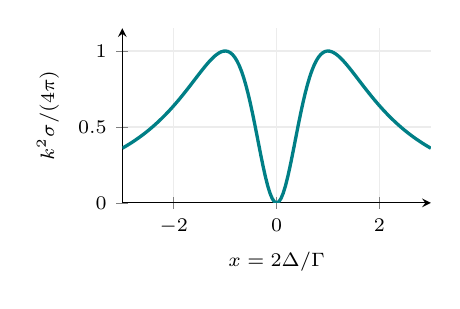
\begin{tikzpicture}
\begin{axis}[width=5.5cm,height=3.8cm,domain=-3:3,samples=141,
axis lines=left,xlabel={$x=2\Delta/\Gamma$},ylabel={$k^2\sigma/(4\pi)$},
xmin=-3,xmax=3,ymin=0,ymax=1.15,xtick={-2,0,2},ytick={0,.5,1},
tick label style={font=\scriptsize},label style={font=\scriptsize},
grid=major,grid style={gray!15}]
\addplot[teal,very thick]{4*x*x/(1+x*x)^2};
\end{axis}
\end{tikzpicture}
\par\scriptsize Analytic illustration: constant width, one channel, no background.
\end{column}
\end{columns}
\src{Thesis, Eqs. 2.212--2.216, pp. 94--96; here using lower-half-plane poles. The curve is an analytic illustration, not thesis data.}
\note{This is a confirmed printed equation error; it does not prove the computed cross sections used the erroneous formula. The inverse S-factor convention gives the same modulus on the real axis. Pole-sign and phase conventions should be made consistent with outgoing poles in the lower half-plane. A multichannel EP does not generally imply that each elastic element is the square of a single-channel scalar, nor a background-independent exact central zero. Ask the candidate to state the conditions under which the model illustration applies.}
\end{frame}

\begin{frame}{Corrections and qualifications to raise proportionately}
\small
\renewcommand{\arraystretch}{1.25}
\begin{tabular}{p{.20\textwidth}p{.71\textwidth}}
\toprule
Eq. 2.210, p. 94 & With residues $c_0,c_1$ defined in the resolvent, the pole amplitude is $(c_0-i c_1t/\hbar)e^{-izt/\hbar}$. A redefinition of $c_1$ must be explicit.\\
Fig. 3.37 / p. 150 & The plotted $d+d$ weight is roughly $+0.05$ to $-0.02$, not within $2\times10^{-3}$ of zero.\\
Table 3.5 / p. 144 & Upper $2^-$ width differs by a factor 1.84; the stated maximum is 1.6. The promised markers of fitted levels are absent.\\
Channel lists & $\nuc{4}{H}\rightarrow\nuc{4}{He}$ and $\alpha\,{}^3G_4\rightarrow{}^1G_4$ on p. 134; ${}^3P_3$ is impossible for $L=S=1$ (pp. 116, 134).\\
Physical wording & Qualify ``probability'', ``unique experimental fingerprint'', ``decoupled from the continuum'', and claims that general $R$-matrix descriptions cannot represent the physics.\\\bottomrule
\end{tabular}
\takeaway{Printed errors, numerical validation gaps and unsettled physical interpretations are different levels of concern.}
\src{Thesis, locations above; see also pp. 7, 126, 129, 147--154, 157--158.}
\note{The amplitude correction assumes exactly the same c1 as in the preceding resolvent expansion; it can be harmless if the author silently redefined it. The cross-section error is a more definite algebraic issue. The channel list likely intends 3P2. Additional precision issues include the HO-CM factorisation on pp.65--66: a complete Nmax space includes CM-excited sectors; tensor factorisation with a CM 0s state applies to the selected physical sector. Exact Lawson shifts require exact factorisation and cannot simultaneously be claimed for a noncommuting truncated Hamiltonian. These wording issues should be addressed without claiming that numerical results are thereby disproved.}
\end{frame}

\begin{frame}{Overall strengths and defence priorities}
\small
\begin{columns}[T]
\begin{column}{.47\textwidth}
\textbf{Scientific strengths}
\begin{itemize}\setlength\itemsep{1mm}
\item Consistent microscopic treatment of open nuclear systems.
\item Several complementary EP diagnostics.
\item Instructive mirror and channel comparisons.
\item Explicit partial widths and model-space study.
\item Reported failures reveal concrete limitations.
\end{itemize}
\end{column}
\begin{column}{.49\textwidth}
\textbf{Priority discussion}
\begin{itemize}\setlength\itemsep{1mm}
\item Candidate's individual contribution and novelty.
\item Robustness under fits, truncations and numerical changes.
\item Observability at the physical Hamiltonian.
\item Preparation, positivity and charged-channel tails.
\item Calibrated versus predicted \nuc{4}{He} quantities.
\end{itemize}
\end{column}
\end{columns}
\takeaway{Connect the model diagnostics to finite, reproducible nuclear observables and decisive experiments.}
\src{Synthesis of Chs. 2--4. Assessment is based on the manuscript; original code and experimental data were not reanalysed.}
\note{There is no need to turn every clarification into a prerequisite for a thesis verdict. The strongest issues are the physical significance of the retuned EPs, time-evolution interpretation and helium calibration. The small notational corrections can be handled quickly. A good defence will explicitly narrow claims, explain the methodological controls and propose decisive additional calculations or experiments.}
\end{frame}

\begin{frame}{Sources and reading conventions}
\small
\begin{itemize}\setlength\itemsep{1.5mm}
\item \textbf{Primary source:} David Cardona Ochoa, \emph{Systematics studies of the continuum-coupling correlations in near-threshold states}, Universit\'e de Caen Normandie, 11 August 2026; supplied final PDF.
\item Page references use \textbf{printed thesis pages}: Arabic page $n$ is PDF page $n+14$. Figure and table labels refer to the thesis.
\item Cardona Ochoa, P\l{}oszajczak and Michel, \emph{Gamow shell model description of exceptional point in $^7$Li}, EPJ Web Conf. \textbf{342}, 01023 (2025). \href{https://arxiv.org/abs/2510.01928}{arXiv:2510.01928}.
\item Cardona Ochoa et al., \emph{Double pole $S$-matrix singularity in the continuum of $^7$Be}, Acta Phys. Pol. B Proc. Suppl. \textbf{19}, 1-A1 (2026). \href{https://arxiv.org/abs/2510.27293}{arXiv:2510.27293}.
\item Wang, Nazarewicz, Volya and Ma, \emph{Probing the Non-exponential Decay Regime in Open Quantum Systems}, Phys. Rev. Research \textbf{5}, 023183 (2023). \href{https://arxiv.org/html/2211.11619}{Full text}.
\item Descouvemont and Baye, \emph{The $R$-matrix theory}, Rep. Prog. Phys. \textbf{73}, 036301 (2010). \href{https://arxiv.org/abs/1001.0678}{arXiv:1001.0678}.
\end{itemize}
\note{The sources beyond the thesis are primary papers or a technical review and support narrowly targeted checks. Numerical experimental values in the slides are taken from the thesis, not a fresh reassessment of evaluated data. The source file contains private opponent notes; the standard PDF displays only the slides. The twelve questions follow at the end, with no subsequent appendix to interrupt that ordering.}
\end{frame}

\section{Twelve questions for the candidate}

\begin{frame}{Defence questions 1--2: contribution and EP identification}
\qtitle{1}{What is your most important original scientific contribution?}
\par Which result goes beyond previously known EP behaviour or earlier GSM--CC work, and which parts of the method and implementation are specifically yours?
\bigskip
\qtitle{2}{How do you establish defectiveness, rather than a close degeneracy?}
\par Explain how eigenvector coalescence, vanishing phase rigidity, square-root splitting and loop exchange support the EP claim. Which test is decisive numerically?
\src{Q1: Introduction, pp. 1--8; Conclusions, pp. 156--159. Q2: pp. 79--94; Figs. 3.3--3.5, 3.13--3.17.}
\note{Q1 purpose: assess ownership and judgement. A strong answer distinguishes the inherited GSM--CC framework, generic Jordan-block theory, the candidate's parameter searches/diagnostics and the new systematics or no-core applications. Do not require novelty of EP theory itself. Follow-up: which single thesis figure best expresses the original physics? Q2 purpose: test mathematical understanding. Look for one eigenvector and a generalised eigenvector at a second-order EP, self-orthogonality, local branch structure and two-loop return. Follow-up: how are phase-rigidity zeros resolved in finite precision, and was a Jordan chain or second-order residue computed directly?}
\end{frame}

\begin{frame}{Defence questions 3--4: robustness and physical relevance}
\qtitle{3}{What uncertainty would you attach to the EP locations?}
\par How do the coordinates and predicted signatures change under continuum-contour refinement, channel-space enlargement and alternative fits of comparable quality?
\bigskip
\qtitle{4}{What does the tuned \nuc{6}{Li} EP tell us about the physical nucleus?}
\par The EP requires roughly doubling the spin--orbit strengths while the starting widths are much too small. Which conclusions survive that distance from the calibrated Hamiltonian?
\src{Q3: model definitions and EP scans, pp. 103--138. Q4: Table 3.1, p. 103; Figs. 3.2--3.4, pp. 104--106.}
\note{Q3 purpose: separate numerical precision from model uncertainty. Look for stable poles under contour deformation and discretisation, channel convergence, fitting covariance, and uncertainty in pole residues/observables. At an EP, eigenvalues are highly sensitive, so extra digits are not an uncertainty estimate. Follow-up: could an acceptable change eliminate or move the relevant EP far away? For 8Be, how are complex channel corrections justified, what flux checks are performed, and how is a threshold-opening effect separated from an EP effect? Q4 purpose: distinguish continuation of an effective Hamiltonian from physical tunability. A good answer accepts the limited quantitative agreement and explains generic structural insights, possible isotope/systematics controls, and realistic pole extraction. Follow-up: repeat the search after fitting widths; is the physical Hamiltonian still near the EP?}
\end{frame}

\begin{frame}{Defence questions 5--6: finite responses and observability}
\qtitle{5}{What physical quantity replaces a divergent pole strength?}
\par Near the EP, individual spectroscopic factors and $B(E2)$ quantities become singular. How would you construct a finite measurable response from the coalescing states and continuum?
\bigskip
\qtitle{6}{What measurement distinguishes an EP from two interfering poles?}
\par Are a split peak and a $2\pi$ phase evolution sufficient? State the conditions behind the ideal double-pole formula and explain the role of Coulomb background and other channels.
\src{Q5: pp. 106--108, 121--125; Figs. 3.6, 3.18--3.21. Q6: pp. 94--99, 125--127; Eq. 2.216; Figs. 3.22--3.23.}
\note{Q5 purpose: test the difference between biorthogonal pole diagnostics and observables. Look for the combined subspace, interference, background continuum and correct metric; a response should not be interpreted through two independently normalised singular eigenvectors. Follow-up: is the finite summed spectroscopic factor itself an observable or only a regular diagnostic? Q6 purpose: test falsifiability. The total phase change alone is not unique. A strong proposal includes a constrained multichannel S-matrix, analytic continuation and pole/residue uncertainties, specified scattering angle and backgrounds, plus a competing non-EP fit. Ask the candidate to derive the positive denominator in Eq.2.216 and confirm which expression the numerical curves used. General multilevel R-matrix approaches should not be equated with isolated Breit--Wigner sums.}
\end{frame}

\begin{frame}{Defence questions 7--8: mirror channels and decay dynamics}
\qtitle{7}{What drives the mirror-channel alignment and width bifurcation?}
\par Separate the roles of Coulomb, thresholds and independently fitted couplings. Why can the trapped \nuc{7}{Be} state retain proton decay while losing its \nuc{3}{He} width?
\bigskip
\qtitle{8}{What physical preparation is represented by your survival curves?}
\par Explain the cutoff packet, negative reconstructed spectra and the polynomial EP envelope. What validates positivity and the evolution near a defective Hamiltonian?
\src{Q7: pp. 117--130; Figs. 3.23--3.28. Q8: Eqs. 2.142, 2.158--2.160, 2.210; Figs. 3.8--3.10, 3.29--3.31.}
\note{Q7 purpose: probe channel-specific decoupling, not an all-or-nothing superradiance analogy. Look for partial-width amplitudes, rank/structure of continuum coupling, changed penetrabilities and mirror fit dependence. The equal EP widths are not symmetry-protected. Follow-up: how robust is near-exclusive branching under additional channels and correction-factor uncertainty? Q8 purpose: establish the physical meaning of the time calculation. A strong answer identifies a reaction-compatible preparation, a positive real-energy spectral measure or explicitly different response, cutoff/diffuseness convergence, and stable matrix-exponential/Jordan propagation. Follow-up: the coefficient b in (a+bt) depends on preparation, so what establishes that the weak beryllium polynomial is caused by the extra channel? A coherent two-pole amplitude contains interference unless averaged or negligible. The resolvent c1 requires -i/hbar in the time amplitude unless redefined.}
\end{frame}

\begin{frame}{Defence questions 9--10: asymptotics and no-core calibration}
\qtitle{9}{Which threshold produces the reported $t^{-5}$ tail?}
\par The open $\alpha+d$ and $\alpha+t$ channels have relative $L=2$ and $L=3$ and contain Coulomb. Can you derive the tail from the calculated threshold density and demonstrate its asymptotic convergence?
\bigskip
\qtitle{10}{What is predictive in the corrected \nuc{4}{He} calculation?}
\par Specify the NN interaction and any three-body terms. After placing thresholds and fitting five energies, how do you assess unfitted widths and the large $2^-$ deuteron correction?
\src{Q9: pp. 72--78, 112, 130; Figs. 3.11, 3.29; Wang et al. (2023), Eq. (5). Q10: pp. 139--145; Tables 3.3--3.6.}
\note{Q9 purpose: separate internal p-wave composition from asymptotic fragment motion. A good answer identifies the actual branch point/edge, includes Coulomb or explains a numerical surrogate, and shows local slopes versus time window, continuum resolution and preparation. Do not demand a neutral t^-7 or t^-9 replacement for a charged calculation. Q10 purpose: assess calibration honestly. Expected information includes potential name, regulator/cutoff, transformation/renormalisation and 3N treatment. Ground state and 1-minus upper position are unfitted; widths and branchings are also unfitted but strongly energy-dependent. Follow-up: compare at a common model space, vary the fitted factors and separate kinematic from wavefunction improvement. The c_d=0.39674 factor is substantial.}
\end{frame}

\begin{frame}{Defence questions 11--12: omitted channels and correlation energy}
\qtitle{11}{How are spurious states distinguished from missing cluster physics?}
\par What norm and centre-of-mass diagnostics justify discarding the deuteron-associated states? Could target excitations or the $N_{\rm CM}\leq2$ restriction explain the missing $1^-_2$ deuteron branch?
\bigskip
\qtitle{12}{How would you define and test the continuum correlation energy?}
\par In the threshold scan, what operator changes and what is the reference? Propose a controlled calculation that isolates the continuum contribution and an observable that could validate it.
\src{Q11: pp. 65--69, 140--146, 150; Fig. 3.36; Table 3.6. Q12: pp. 147--154; Figs. 3.37--3.41.}
\note{Q11 purpose: test whether a convergence sequence excludes relevant physical configurations. Look for norm eigenvalues, Pauli redundancy, CM expectation/distribution, cutoff dependence and enlargement of the deuteron/target spaces. Stability under N alone does not prove a state physical or spurious. The raw 1-minus upper deuteron branch is negligible even though the channel is open, so an energy correction alone is insufficient. Q12 purpose: finish with constructive scientific judgement. A strong answer specifies the Hamiltonian deformation, an uncoupled reference or Feshbach self-energy and controlled coupling variation at fixed kinematics. Closed channels contribute real virtual shifts. Channel c-product weights are not positive probabilities; compare pole trajectories, residues, branchings and measured scattering responses. Ask which single proposed calculation or experiment would most decisively strengthen the thesis's interpretation.}
\end{frame}

\end{document}
